\documentclass[twoside]{book}

% Packages required by doxygen
\usepackage{fixltx2e}
\usepackage{calc}
\usepackage{doxygen}
\usepackage[export]{adjustbox} % also loads graphicx
\usepackage{graphicx}
\usepackage[utf8]{inputenc}
\usepackage{makeidx}
\usepackage{multicol}
\usepackage{multirow}
\PassOptionsToPackage{warn}{textcomp}
\usepackage{textcomp}
\usepackage[nointegrals]{wasysym}
\usepackage[table]{xcolor}

% Font selection
\usepackage[T1]{fontenc}
\usepackage[scaled=.90]{helvet}
\usepackage{courier}
\usepackage{amssymb}
\usepackage{sectsty}
\renewcommand{\familydefault}{\sfdefault}
\allsectionsfont{%
  \fontseries{bc}\selectfont%
  \color{darkgray}%
}
\renewcommand{\DoxyLabelFont}{%
  \fontseries{bc}\selectfont%
  \color{darkgray}%
}
\newcommand{\+}{\discretionary{\mbox{\scriptsize$\hookleftarrow$}}{}{}}

% Page & text layout
\usepackage{geometry}
\geometry{%
  a4paper,%
  top=2.5cm,%
  bottom=2.5cm,%
  left=2.5cm,%
  right=2.5cm%
}
\tolerance=750
\hfuzz=15pt
\hbadness=750
\setlength{\emergencystretch}{15pt}
\setlength{\parindent}{0cm}
\setlength{\parskip}{3ex plus 2ex minus 2ex}
\makeatletter
\renewcommand{\paragraph}{%
  \@startsection{paragraph}{4}{0ex}{-1.0ex}{1.0ex}{%
    \normalfont\normalsize\bfseries\SS@parafont%
  }%
}
\renewcommand{\subparagraph}{%
  \@startsection{subparagraph}{5}{0ex}{-1.0ex}{1.0ex}{%
    \normalfont\normalsize\bfseries\SS@subparafont%
  }%
}
\makeatother

% Headers & footers
\usepackage{fancyhdr}
\pagestyle{fancyplain}
\fancyhead[LE]{\fancyplain{}{\bfseries\thepage}}
\fancyhead[CE]{\fancyplain{}{}}
\fancyhead[RE]{\fancyplain{}{\bfseries\leftmark}}
\fancyhead[LO]{\fancyplain{}{\bfseries\rightmark}}
\fancyhead[CO]{\fancyplain{}{}}
\fancyhead[RO]{\fancyplain{}{\bfseries\thepage}}
\fancyfoot[LE]{\fancyplain{}{}}
\fancyfoot[CE]{\fancyplain{}{}}
\fancyfoot[RE]{\fancyplain{}{\bfseries\scriptsize Generated by Doxygen }}
\fancyfoot[LO]{\fancyplain{}{\bfseries\scriptsize Generated by Doxygen }}
\fancyfoot[CO]{\fancyplain{}{}}
\fancyfoot[RO]{\fancyplain{}{}}
\renewcommand{\footrulewidth}{0.4pt}
\renewcommand{\chaptermark}[1]{%
  \markboth{#1}{}%
}
\renewcommand{\sectionmark}[1]{%
  \markright{\thesection\ #1}%
}

% Indices & bibliography
\usepackage{natbib}
\usepackage[titles]{tocloft}
\setcounter{tocdepth}{3}
\setcounter{secnumdepth}{5}
\makeindex

% Hyperlinks (required, but should be loaded last)
\usepackage{ifpdf}
\ifpdf
  \usepackage[pdftex,pagebackref=true]{hyperref}
\else
  \usepackage[ps2pdf,pagebackref=true]{hyperref}
\fi
\hypersetup{%
  colorlinks=true,%
  linkcolor=blue,%
  citecolor=blue,%
  unicode%
}

% Custom commands
\newcommand{\clearemptydoublepage}{%
  \newpage{\pagestyle{empty}\cleardoublepage}%
}

\usepackage{caption}
\captionsetup{labelsep=space,justification=centering,font={bf},singlelinecheck=off,skip=4pt,position=top}

%===== C O N T E N T S =====

\begin{document}

% Titlepage & ToC
\hypersetup{pageanchor=false,
             bookmarksnumbered=true,
             pdfencoding=unicode
            }
\pagenumbering{alph}
\begin{titlepage}
\vspace*{7cm}
\begin{center}%
{\Large Personelle Management \\[1ex]\large 1.\+0.\+1 }\\
\vspace*{1cm}
{\large Generated by Doxygen 1.8.14}\\
\end{center}
\end{titlepage}
\clearemptydoublepage
\pagenumbering{roman}
\tableofcontents
\clearemptydoublepage
\pagenumbering{arabic}
\hypersetup{pageanchor=true}

%--- Begin generated contents ---
\chapter{User\+Login\+App}
\label{md__r_e_a_d_m_e}
\Hypertarget{md__r_e_a_d_m_e}
Simple app with S\+Q\+L\+I\+TE backend for user manipulation

This app demonstarte how we can use S\+Q\+L\+I\+TE database as a backend for our Q\+ML application by using Local\+Storage module from Qt.

This demo app has following feature implemented.
\begin{DoxyItemize}
\item User registration
\item User login
\item Password retrievel
\end{DoxyItemize}

Icons used in this app are from Font Awesome \mbox{[}\href{http://fontawesome.io/icons/}{\tt http\+://fontawesome.\+io/icons/}\mbox{]}

Screenshots\+:

Log\+In Screen\+:



Register Screen\+:



Password Reset Screen\+:



User\+Info Screen\+:

 
\chapter{Hierarchical Index}
\section{Class Hierarchy}
This inheritance list is sorted roughly, but not completely, alphabetically\+:\begin{DoxyCompactList}
\item Q\+Object\begin{DoxyCompactList}
\item \contentsline{section}{Data\+Base}{\pageref{class_data_base}}{}
\end{DoxyCompactList}
\item Q\+Sql\+Query\+Model\begin{DoxyCompactList}
\item \contentsline{section}{Con\+Model}{\pageref{class_con_model}}{}
\item \contentsline{section}{List\+Model}{\pageref{class_list_model}}{}
\item \contentsline{section}{Sales\+Model}{\pageref{class_sales_model}}{}
\end{DoxyCompactList}
\end{DoxyCompactList}

\chapter{Class Index}
\section{Class List}
Here are the classes, structs, unions and interfaces with brief descriptions\+:\begin{DoxyCompactList}
\item\contentsline{section}{\mbox{\hyperlink{class_con_model}{Con\+Model}} }{\pageref{class_con_model}}{}
\item\contentsline{section}{\mbox{\hyperlink{class_data_base}{Data\+Base}} }{\pageref{class_data_base}}{}
\item\contentsline{section}{\mbox{\hyperlink{class_list_model}{List\+Model}} }{\pageref{class_list_model}}{}
\item\contentsline{section}{\mbox{\hyperlink{class_sales_model}{Sales\+Model}} }{\pageref{class_sales_model}}{}
\end{DoxyCompactList}

\chapter{Class Documentation}
\hypertarget{class_con_model}{}\section{Con\+Model Class Reference}
\label{class_con_model}\index{Con\+Model@{Con\+Model}}
Inheritance diagram for Con\+Model\+:\begin{figure}[H]
\begin{center}
\leavevmode
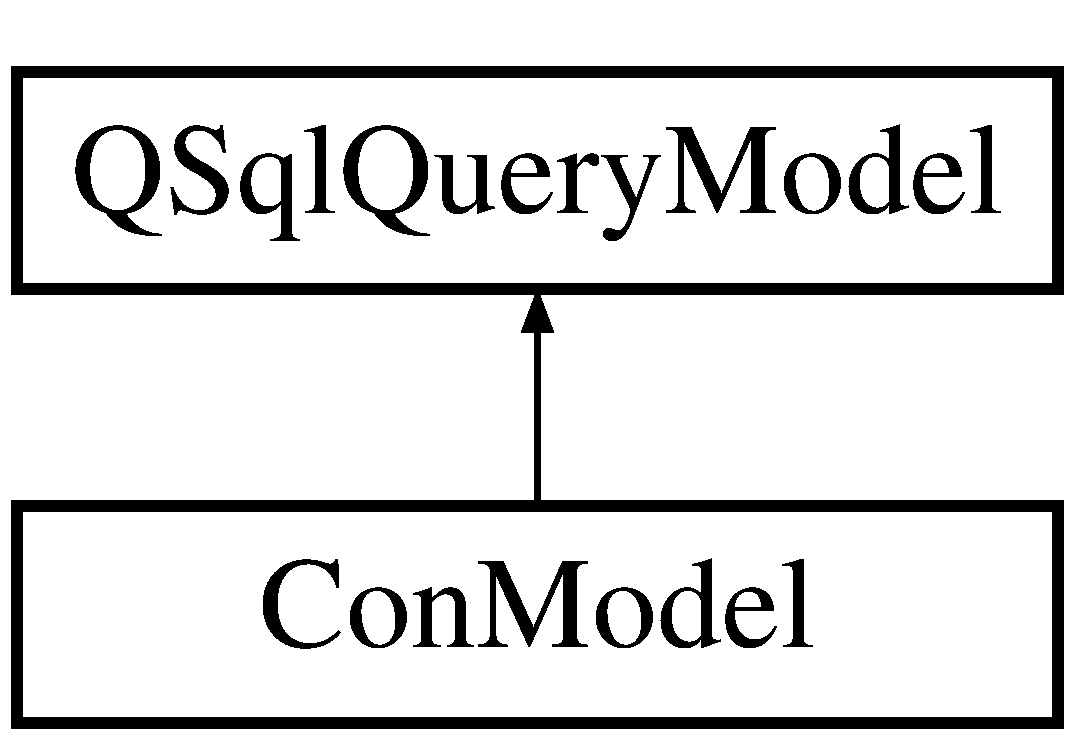
\includegraphics[height=2.000000cm]{class_con_model}
\end{center}
\end{figure}
\subsection*{Public Types}
\begin{DoxyCompactItemize}
\item 
\mbox{\Hypertarget{class_con_model_a7fc2a548f548de69b4b31b3c0e3fe7e4}\label{class_con_model_a7fc2a548f548de69b4b31b3c0e3fe7e4}} 
enum {\bfseries Roles} \{ \newline
{\bfseries Id\+Role} = Qt\+:\+:User\+Role + 1, 
{\bfseries Name\+Role}, 
{\bfseries Department\+Role}, 
{\bfseries Work\+Hrs\+Day\+Role}, 
\newline
{\bfseries Monthly\+Salary\+Role}
 \}
\end{DoxyCompactItemize}
\subsection*{Public Slots}
\begin{DoxyCompactItemize}
\item 
\mbox{\Hypertarget{class_con_model_a6ee8067e3ac42b99c0bb4969a3b68a3f}\label{class_con_model_a6ee8067e3ac42b99c0bb4969a3b68a3f}} 
void {\bfseries update\+Model} ()
\item 
\mbox{\Hypertarget{class_con_model_aa1490599f379abb6f838e1ac18841293}\label{class_con_model_aa1490599f379abb6f838e1ac18841293}} 
void {\bfseries update\+Data} ()
\item 
\mbox{\Hypertarget{class_con_model_a7825b4bc4bfdcdd0404f9186b1413f6e}\label{class_con_model_a7825b4bc4bfdcdd0404f9186b1413f6e}} 
int {\bfseries get\+Id} (int row)
\item 
\mbox{\Hypertarget{class_con_model_aa126b22b4b25e28a2115a8b19c233f4a}\label{class_con_model_aa126b22b4b25e28a2115a8b19c233f4a}} 
Q\+String {\bfseries get\+Name} (int row)
\item 
\mbox{\Hypertarget{class_con_model_af39cb5e003655e73f392f4eba3af79b9}\label{class_con_model_af39cb5e003655e73f392f4eba3af79b9}} 
Q\+String {\bfseries get\+Department} (int row)
\item 
\mbox{\Hypertarget{class_con_model_a01dcfaacf11f32348f479367282fc832}\label{class_con_model_a01dcfaacf11f32348f479367282fc832}} 
Q\+String {\bfseries get\+Work\+Hrs\+Day} (int row)
\item 
\mbox{\Hypertarget{class_con_model_ac124e2a925ed61f670b5965b63d1e3ae}\label{class_con_model_ac124e2a925ed61f670b5965b63d1e3ae}} 
Q\+String {\bfseries get\+Monthly\+Salary} (int row)
\end{DoxyCompactItemize}
\subsection*{Public Member Functions}
\begin{DoxyCompactItemize}
\item 
\mbox{\Hypertarget{class_con_model_a9c45f9fcdc6b8cdd61f214dbd8bb5c0a}\label{class_con_model_a9c45f9fcdc6b8cdd61f214dbd8bb5c0a}} 
{\bfseries Con\+Model} (Q\+Object $\ast$parent=0)
\item 
\mbox{\Hypertarget{class_con_model_a1aee4378113c58fa0d3906b3a1b93b9d}\label{class_con_model_a1aee4378113c58fa0d3906b3a1b93b9d}} 
Q\+Variant {\bfseries data} (const Q\+Model\+Index \&index, int role=Qt\+::\+Display\+Role) const
\end{DoxyCompactItemize}
\subsection*{Protected Member Functions}
\begin{DoxyCompactItemize}
\item 
\mbox{\Hypertarget{class_con_model_a9752bc78332c8ef9b2fe65af3c30afc8}\label{class_con_model_a9752bc78332c8ef9b2fe65af3c30afc8}} 
Q\+Hash$<$ int, Q\+Byte\+Array $>$ {\bfseries role\+Names} () const
\end{DoxyCompactItemize}


\subsection{Detailed Description}


Definition at line 9 of file contract.\+h.



The documentation for this class was generated from the following files\+:\begin{DoxyCompactItemize}
\item 
headers/contract.\+h\item 
sources/contract.\+cpp\end{DoxyCompactItemize}

\hypertarget{class_data_base}{}\section{Data\+Base Class Reference}
\label{class_data_base}\index{Data\+Base@{Data\+Base}}
Inheritance diagram for Data\+Base\+:\begin{figure}[H]
\begin{center}
\leavevmode
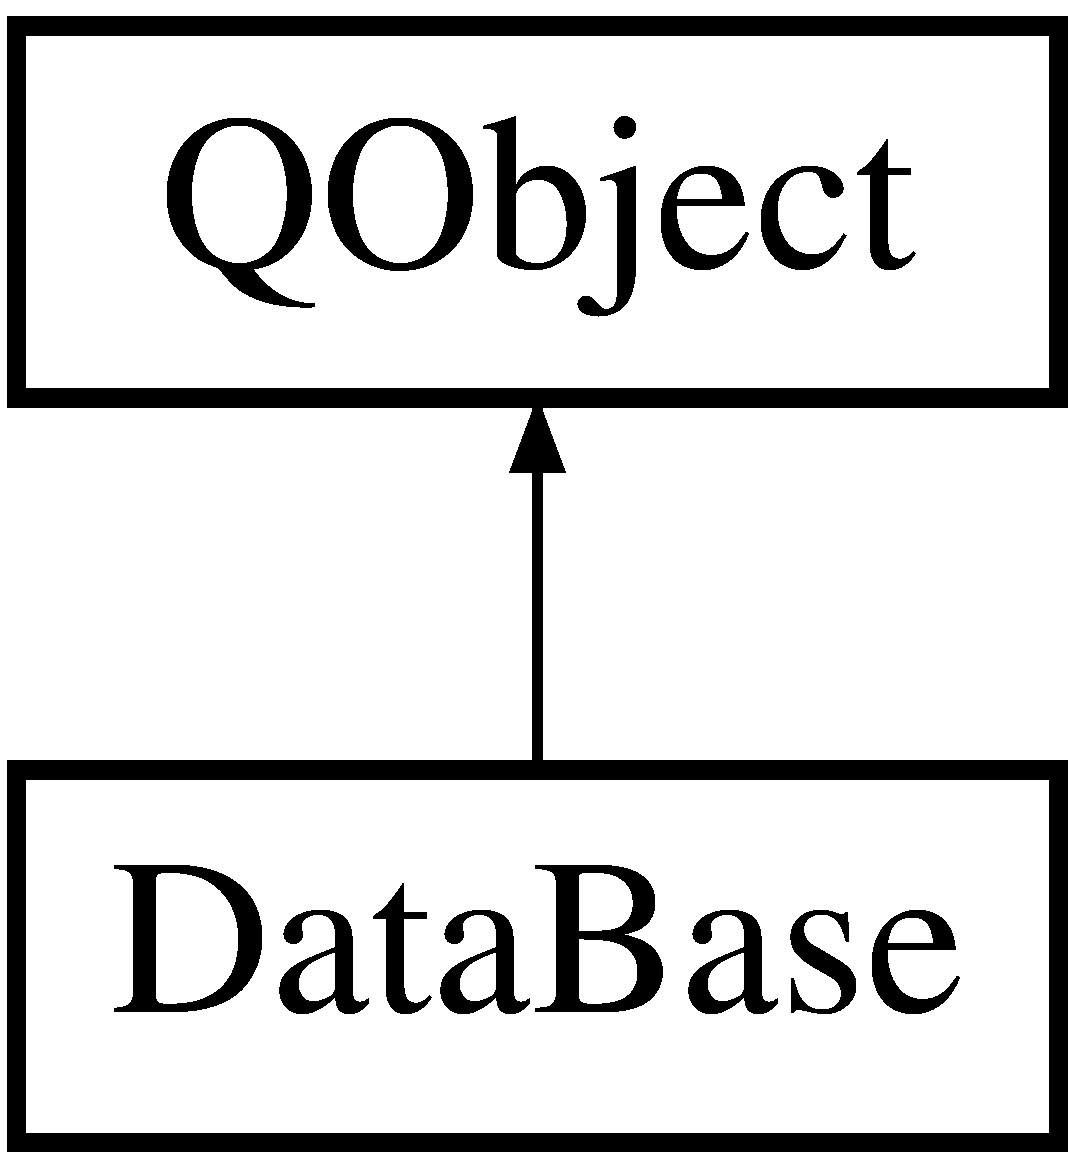
\includegraphics[height=2.000000cm]{class_data_base}
\end{center}
\end{figure}
\subsection*{Public Slots}
\begin{DoxyCompactItemize}
\item 
\mbox{\Hypertarget{class_data_base_af4874270775a567003c3e0295bd13da4}\label{class_data_base_af4874270775a567003c3e0295bd13da4}} 
bool {\bfseries inser\+Into\+Table} (const int id, const Q\+String \&name, const Q\+String \&department, const Q\+String \&gender, const Q\+String \&job\+\_\+position)
\item 
\mbox{\Hypertarget{class_data_base_a383a66d485d39b99dffc81736b9ef99e}\label{class_data_base_a383a66d485d39b99dffc81736b9ef99e}} 
bool {\bfseries update} (const int id, const Q\+String \&name, const Q\+String \&department, const Q\+String \&gender, const Q\+String \&job\+\_\+position)
\item 
\mbox{\Hypertarget{class_data_base_a6ef1a8a1ce8133ac9d8e56366f5e1395}\label{class_data_base_a6ef1a8a1ce8133ac9d8e56366f5e1395}} 
bool {\bfseries remove\+Record} (const int id)
\item 
\mbox{\Hypertarget{class_data_base_a7831da5caf873d7e4636f8131f5c397d}\label{class_data_base_a7831da5caf873d7e4636f8131f5c397d}} 
bool {\bfseries insert} (const int id, const Q\+String \&name, const Q\+String \&department, const Q\+String \&workhrsday, const Q\+String \&monthlysalary)
\item 
\mbox{\Hypertarget{class_data_base_a95b09aa60de1c4e0375a58c3cb718ef7}\label{class_data_base_a95b09aa60de1c4e0375a58c3cb718ef7}} 
bool {\bfseries update2} (const int id, const Q\+String \&name, const Q\+String \&department, const Q\+String \&workhrsday, const Q\+String \&monthlysalary)
\item 
\mbox{\Hypertarget{class_data_base_a320efe9c042e576f0e59176603d945d9}\label{class_data_base_a320efe9c042e576f0e59176603d945d9}} 
bool {\bfseries remove} (const int id)
\item 
\mbox{\Hypertarget{class_data_base_a6102263338b25dcc1b49f53d02886c12}\label{class_data_base_a6102263338b25dcc1b49f53d02886c12}} 
bool {\bfseries remove2} (const int id)
\item 
\mbox{\Hypertarget{class_data_base_a462cd3f510fe492783c4b9647f9dcffe}\label{class_data_base_a462cd3f510fe492783c4b9647f9dcffe}} 
bool {\bfseries insert2} (const int id, const Q\+String \&name, const Q\+String \&phone, const Q\+String \&product, const Q\+String \&workhrsday, const Q\+String \&monthlysalary)
\item 
\mbox{\Hypertarget{class_data_base_af1ed979251180931a33d71d5681e1466}\label{class_data_base_af1ed979251180931a33d71d5681e1466}} 
bool {\bfseries update3} (const int id, const Q\+String \&name, const Q\+String \&phone, const Q\+String \&product, const Q\+String \&workhrsday, const Q\+String \&monthlysalary)
\end{DoxyCompactItemize}
\subsection*{Signals}
\begin{DoxyCompactItemize}
\item 
\mbox{\Hypertarget{class_data_base_a8890efbd2c70b08529079cd2b45c85ba}\label{class_data_base_a8890efbd2c70b08529079cd2b45c85ba}} 
void {\bfseries error\+Change} ()
\end{DoxyCompactItemize}
\subsection*{Public Member Functions}
\begin{DoxyCompactItemize}
\item 
\mbox{\Hypertarget{class_data_base_af4276b07c4049897ecbfe4842d25ba02}\label{class_data_base_af4276b07c4049897ecbfe4842d25ba02}} 
{\bfseries Data\+Base} (Q\+Object $\ast$parent=0)
\end{DoxyCompactItemize}
\subsection*{Properties}
\begin{DoxyCompactItemize}
\item 
\mbox{\Hypertarget{class_data_base_aef16708ec124b90da338ec222c4dc608}\label{class_data_base_aef16708ec124b90da338ec222c4dc608}} 
bool {\bfseries Connectionerror}
\end{DoxyCompactItemize}


\subsection{Detailed Description}


Definition at line 42 of file database.\+h.



The documentation for this class was generated from the following files\+:\begin{DoxyCompactItemize}
\item 
headers/database.\+h\item 
sources/database.\+cpp\end{DoxyCompactItemize}

\hypertarget{class_list_model}{}\section{List\+Model Class Reference}
\label{class_list_model}\index{List\+Model@{List\+Model}}
Inheritance diagram for List\+Model\+:\begin{figure}[H]
\begin{center}
\leavevmode
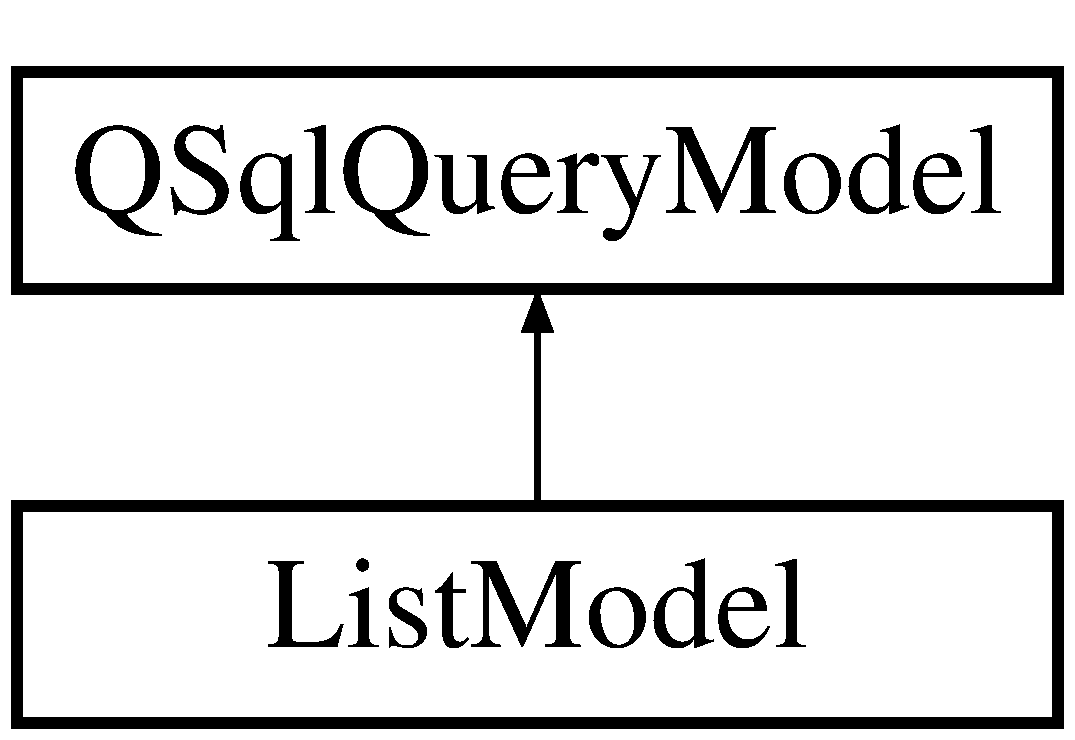
\includegraphics[height=2.000000cm]{class_list_model}
\end{center}
\end{figure}
\subsection*{Public Types}
\begin{DoxyCompactItemize}
\item 
\mbox{\Hypertarget{class_list_model_a878f6de48ea8627511fe16821149bf65}\label{class_list_model_a878f6de48ea8627511fe16821149bf65}} 
enum {\bfseries Roles} \{ \newline
{\bfseries Id\+Role} = Qt\+:\+:User\+Role + 1, 
{\bfseries Name\+Role}, 
{\bfseries Department\+Role}, 
{\bfseries Gender\+Role}, 
\newline
{\bfseries Job\+\_\+position\+Role}
 \}
\end{DoxyCompactItemize}
\subsection*{Public Slots}
\begin{DoxyCompactItemize}
\item 
\mbox{\Hypertarget{class_list_model_aca658eddcc300788b566f3c698b6a296}\label{class_list_model_aca658eddcc300788b566f3c698b6a296}} 
void {\bfseries update\+Model} ()
\item 
\mbox{\Hypertarget{class_list_model_a9671f673440a893fe72b393df53d32f8}\label{class_list_model_a9671f673440a893fe72b393df53d32f8}} 
void {\bfseries update\+Data} ()
\item 
\mbox{\Hypertarget{class_list_model_ad52415be6403eae2c4b5b38bed922fb9}\label{class_list_model_ad52415be6403eae2c4b5b38bed922fb9}} 
int {\bfseries get\+Id} (int row)
\item 
\mbox{\Hypertarget{class_list_model_a418107418cbddf6f96e245df2f3464af}\label{class_list_model_a418107418cbddf6f96e245df2f3464af}} 
Q\+String {\bfseries get\+Name} (int row)
\item 
\mbox{\Hypertarget{class_list_model_a56818d355bcd0978ff89d01327e899d6}\label{class_list_model_a56818d355bcd0978ff89d01327e899d6}} 
Q\+String {\bfseries get\+Department} (int row)
\item 
\mbox{\Hypertarget{class_list_model_ab1396f72e481816fcb30cdf67d90cda4}\label{class_list_model_ab1396f72e481816fcb30cdf67d90cda4}} 
Q\+String {\bfseries get\+Gender} (int row)
\item 
\mbox{\Hypertarget{class_list_model_a5374a643c5726f7ae9157cad07b66703}\label{class_list_model_a5374a643c5726f7ae9157cad07b66703}} 
Q\+String {\bfseries get\+Job\+\_\+position} (int row)
\end{DoxyCompactItemize}
\subsection*{Public Member Functions}
\begin{DoxyCompactItemize}
\item 
\mbox{\Hypertarget{class_list_model_a26cd1a0d21d6015d4847774acfe9a716}\label{class_list_model_a26cd1a0d21d6015d4847774acfe9a716}} 
{\bfseries List\+Model} (Q\+Object $\ast$parent=0)
\item 
\mbox{\Hypertarget{class_list_model_a75ad769eac92db357d5a9fbedd9c2bc4}\label{class_list_model_a75ad769eac92db357d5a9fbedd9c2bc4}} 
Q\+Variant {\bfseries data} (const Q\+Model\+Index \&index, int role=Qt\+::\+Display\+Role) const
\end{DoxyCompactItemize}
\subsection*{Protected Member Functions}
\begin{DoxyCompactItemize}
\item 
\mbox{\Hypertarget{class_list_model_ac58278766ba826b23cc5949fbef16362}\label{class_list_model_ac58278766ba826b23cc5949fbef16362}} 
Q\+Hash$<$ int, Q\+Byte\+Array $>$ {\bfseries role\+Names} () const
\end{DoxyCompactItemize}


\subsection{Detailed Description}


Definition at line 8 of file listmodel.\+h.



The documentation for this class was generated from the following files\+:\begin{DoxyCompactItemize}
\item 
headers/listmodel.\+h\item 
sources/listmodel.\+cpp\end{DoxyCompactItemize}

\hypertarget{class_sales_model}{}\section{Sales\+Model Class Reference}
\label{class_sales_model}\index{Sales\+Model@{Sales\+Model}}
Inheritance diagram for Sales\+Model\+:\begin{figure}[H]
\begin{center}
\leavevmode
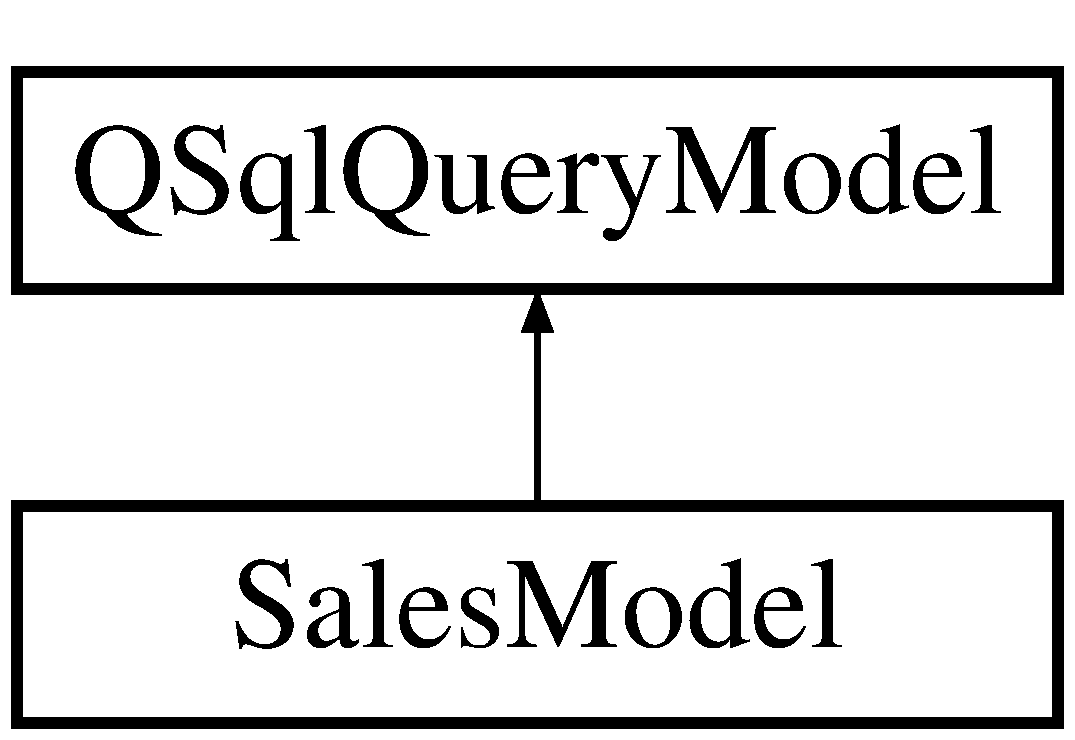
\includegraphics[height=2.000000cm]{class_sales_model}
\end{center}
\end{figure}
\subsection*{Public Types}
\begin{DoxyCompactItemize}
\item 
\mbox{\Hypertarget{class_sales_model_a536c3f3fd1e875635d7cdc2f25128bf3}\label{class_sales_model_a536c3f3fd1e875635d7cdc2f25128bf3}} 
enum {\bfseries Roles} \{ \newline
{\bfseries Id\+Role} = Qt\+:\+:User\+Role + 1, 
{\bfseries Name\+Role}, 
{\bfseries Phone\+Role}, 
{\bfseries Product\+Role}, 
\newline
{\bfseries Work\+Hrs\+Day\+Role}, 
{\bfseries Monthly\+Salary\+Role}
 \}
\end{DoxyCompactItemize}
\subsection*{Public Slots}
\begin{DoxyCompactItemize}
\item 
\mbox{\Hypertarget{class_sales_model_a6947c5eb05b386ca7f09f318a3ae6230}\label{class_sales_model_a6947c5eb05b386ca7f09f318a3ae6230}} 
void {\bfseries update\+Model} ()
\item 
\mbox{\Hypertarget{class_sales_model_a9f0f54cfc8b9f9d59ba61c133d99ce6f}\label{class_sales_model_a9f0f54cfc8b9f9d59ba61c133d99ce6f}} 
int {\bfseries get\+Id} (int row)
\item 
\mbox{\Hypertarget{class_sales_model_a4d5cdac1aef9374008d6acd21a1d7881}\label{class_sales_model_a4d5cdac1aef9374008d6acd21a1d7881}} 
Q\+String {\bfseries get\+Name} (int row)
\item 
\mbox{\Hypertarget{class_sales_model_ac80d9783d2cb2560f0374a60f989562a}\label{class_sales_model_ac80d9783d2cb2560f0374a60f989562a}} 
Q\+String {\bfseries get\+Phone} (int row)
\item 
\mbox{\Hypertarget{class_sales_model_aca8ab7541d3b0c4f865bf1bcae2bff5e}\label{class_sales_model_aca8ab7541d3b0c4f865bf1bcae2bff5e}} 
Q\+String {\bfseries get\+Product} (int row)
\item 
\mbox{\Hypertarget{class_sales_model_ae1a76068ac6f4b8fd26c5e2fe1e41f57}\label{class_sales_model_ae1a76068ac6f4b8fd26c5e2fe1e41f57}} 
Q\+String {\bfseries get\+Work\+Hrs\+Day} (int row)
\item 
\mbox{\Hypertarget{class_sales_model_adfe23e5bd369b7623586eb5dfe7c2a36}\label{class_sales_model_adfe23e5bd369b7623586eb5dfe7c2a36}} 
Q\+String {\bfseries get\+Monthly\+Salary} (int row)
\end{DoxyCompactItemize}
\subsection*{Public Member Functions}
\begin{DoxyCompactItemize}
\item 
\mbox{\Hypertarget{class_sales_model_a230673a20e616d4dcb993acbfe3426e1}\label{class_sales_model_a230673a20e616d4dcb993acbfe3426e1}} 
{\bfseries Sales\+Model} (Q\+Object $\ast$parent=0)
\item 
\mbox{\Hypertarget{class_sales_model_ac6358cf833faababa04458a5cf45b421}\label{class_sales_model_ac6358cf833faababa04458a5cf45b421}} 
Q\+Variant {\bfseries data} (const Q\+Model\+Index \&index, int role=Qt\+::\+Display\+Role) const
\end{DoxyCompactItemize}
\subsection*{Protected Member Functions}
\begin{DoxyCompactItemize}
\item 
\mbox{\Hypertarget{class_sales_model_ae483317481b0f4c68025e10dbd69e4ef}\label{class_sales_model_ae483317481b0f4c68025e10dbd69e4ef}} 
Q\+Hash$<$ int, Q\+Byte\+Array $>$ {\bfseries role\+Names} () const
\end{DoxyCompactItemize}


\subsection{Detailed Description}


Definition at line 10 of file salesman.\+h.



The documentation for this class was generated from the following files\+:\begin{DoxyCompactItemize}
\item 
headers/salesman.\+h\item 
sources/salesman.\+cpp\end{DoxyCompactItemize}

%--- End generated contents ---

% Index
\backmatter
\newpage
\phantomsection
\clearemptydoublepage
\addcontentsline{toc}{chapter}{Index}
\printindex

\end{document}
